\chapter{Uncertainties}\label{chap:uncertBkgmodel}
A central part of the analysis is quantifying the potential bias introduced by the choice of a particular function and quantifying the uncertainty on both the shape and normalisation of the background estimation. The uncertainties related to the background modelling results from three sources: the inherent bias of the function (\cref{sec:uncertBkgmodel:iss}), statistical uncertainty of the fit (\cref{sec:uncertBkgmodel:statu}) and the residual difference between the signal+background and the background-only functions (\cref{sec:uncertBkgmodel:crbu}). The uncertainties are estimated using the background-only function, as it is used for the final background estimate in data. 

The interpretation of the results in the context of CI model uses the MC templates, described in \cref{chap:stats}. Therefore, the uncertainties associated with the simulated samples are also quantified for the SR choices considered in the analysis (\cref{sec:uncertBkgmodel:signalyield}).
 
\section{Background estimate uncertainties}

\subsection{Induced spurious-signal uncertainty}\label{sec:uncertBkgmodel:iss}
For a given underlying PDF that generates an invariant mass spectrum, the extrapolation from the low-mass CR to the high-mass SR will naturally deviate from the underlying distribution, resulting in an excess or deficit compared to the background template. The \emph{induced spurious-signal} uncertainty (\ISSU) quantifies the amount to which the background function, when extrapolated to the SR can induce a signal-like excess or deficit. 

At high mass the underlying background distribution in data is not known accurately. A \ISSU measurement made on the template from only the nominal PDF would assume the underlying distribution to be known precisely. Therefore, the theoretical uncertainties associated with the nominal PDF choice described in \cref{sec:sysmc:theory} are also considered in the \ISSU measurement. Additionally, due to detector and reconstruction effects on the simulated MC template, the experimental uncertainties, described in \cref{sec:sysmc:exp}, are also considered. 

The \ISSU is measured on the nominal MC background, and its systematic variations. An ensemble of possible simulated shapes are created scaling the nominal simulated background template by a linear combination of all of its systematic uncertainties. Each uncertainty is scaled by a Gaussian factor in the range [-1,1], summed together, and used to scale the simulated background shape to produce a toy distribution. \cref{eq:issutoy} outlines the procedure used to construct each toy background shape. 
\begin{equation}
    \label{eq:issutoy}
    \begin{aligned}
        & Toy = \sum_{i} N_{bkg,i} + \sum_{j} \left(\delta_{i,j} * \alpha_{j}\right), \\
        & \alpha_j = \mathrm{Gaus}(\sigma=1,\mu=0),
    \end{aligned}
\end{equation}
where $N_{bkg,i}$ is the number of background events in invariant mass bin \emph{i} for the nominal simulated background distribution, $\delta_{i,j}$ is the uncertainty for background uncertainty \emph{j}, and $\alpha_j$ is a factor sampled from a gaussian distribution used to scale each uncertainty.

The resulting toy shape is fitted and extrapolated to the SR. The difference between the integral of the extrapolation and the toy background in the SR is taken as the induced spurious signal per toy. The induced spurious-signal is calculated for each toy in the ensemble of toys, producing a distribution for induced spurious-signal values. The sum in quadrature of the mean and standard deviation of the induced spurious-signal distribution is taken as the \ISSU. 

The induced spurious signal distributions, as event yields in the SR, for the CR and SRs considered in the analysis is shown in \cref{fig:bkgmodel:issu}. A set 10000 toy uncertainty templates are made and fit using the background-only function. The induced spurious signal for each toy is calculated to form the distribution. The standard deviation and the mean for each CR and SR configuration is calculated from the spurious signal distribution to determine the \ISSU. The choice of 10000 toys is deemed appropriate as the mean, and standard deviation of the distributions are found to be consistent stable up to 0.001\% when comparing with distributions with 9000 toys.

\begin{figure}[h!]
    \centering
    \begin{subfigure}[b]{0.49\textwidth}
        \centering
        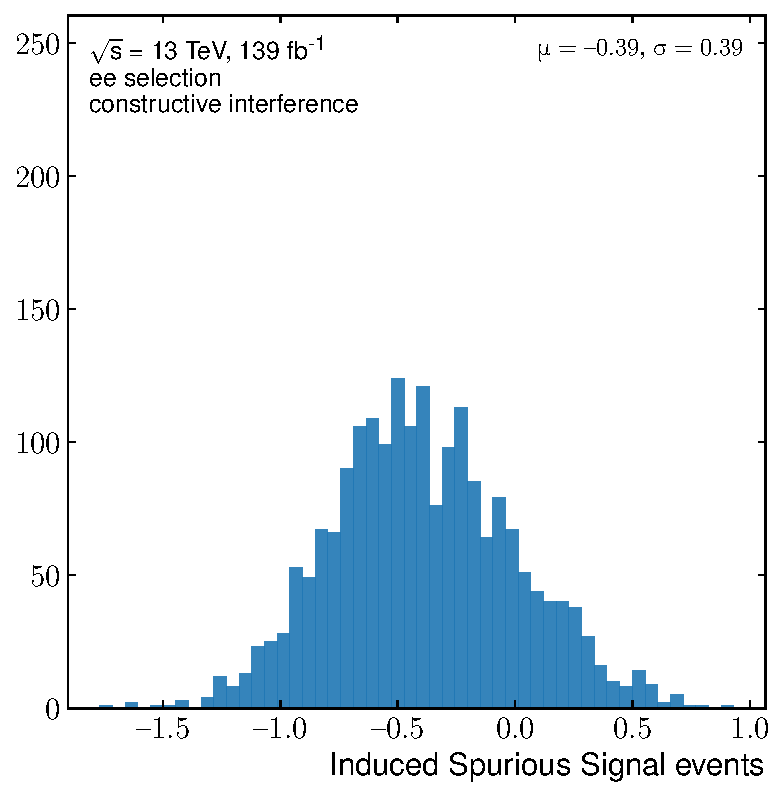
\includegraphics[width=\textwidth]{/Users/Deshan/Documents/PhD/thesis/Thesis/figures/analysis/bkgmodel/uncertainties/toyNSSDist-ee-const-all-noGaus.pdf}
        \label{fig:bkgmodel:issu1}
    \end{subfigure}
    \begin{subfigure}[b]{0.49\textwidth}
        \centering
        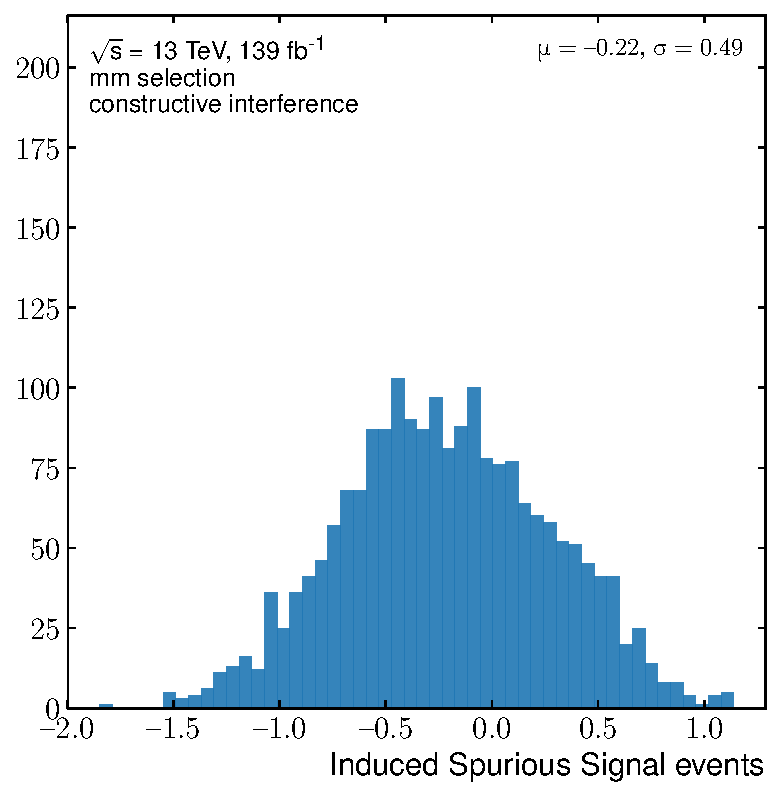
\includegraphics[width=\textwidth]{/Users/Deshan/Documents/PhD/thesis/Thesis/figures/analysis/bkgmodel/uncertainties/toyNSSDist-mm-const-all-noGaus.pdf}
        \label{fig:bkgmodel:issu2}
    \end{subfigure}
    \begin{subfigure}[b]{0.49\textwidth}
        \centering
        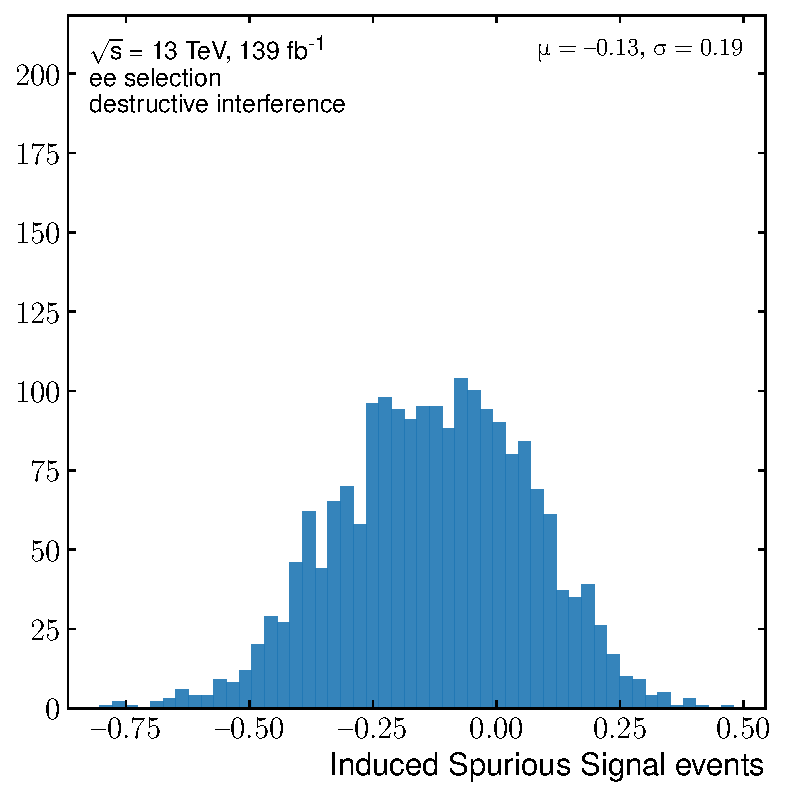
\includegraphics[width=\textwidth]{/Users/Deshan/Documents/PhD/thesis/Thesis/figures/analysis/bkgmodel/uncertainties/toyNSSDist-ee-dest-all-noGaus.pdf}
        \label{fig:bkgmodel:issu3}
    \end{subfigure}
    \begin{subfigure}[b]{0.49\textwidth}
        \centering
        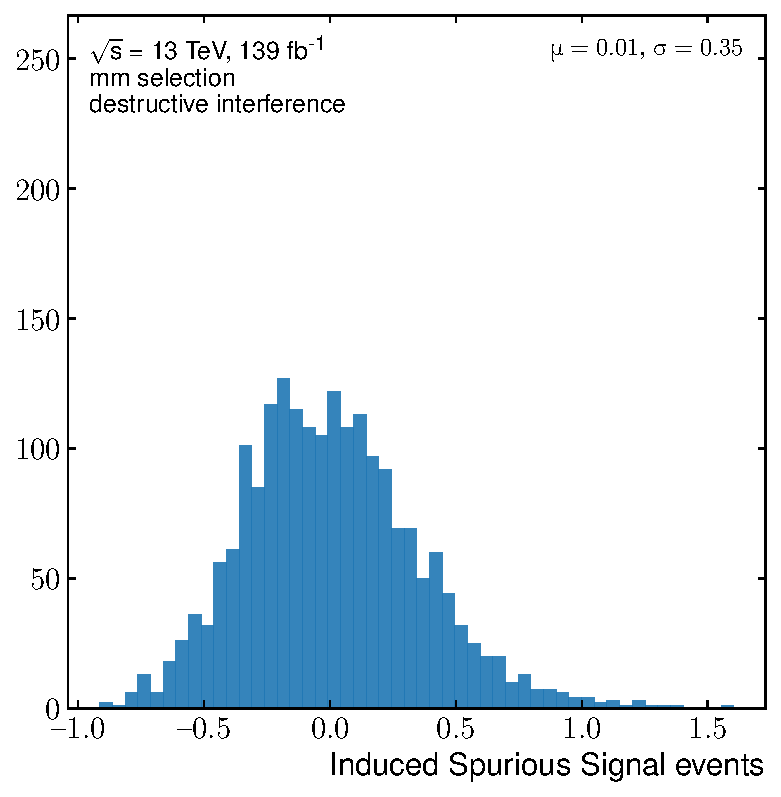
\includegraphics[width=\textwidth]{/Users/Deshan/Documents/PhD/thesis/Thesis/figures/analysis/bkgmodel/uncertainties/toyNSSDist-mm-dest-all-noGaus.pdf}
        \label{fig:bkgmodel:issu4}
    \end{subfigure}
    \caption[Induced spurious signal distributions from fits to toy uncertainties.]{Distribution of induced spurious signal values, as number of events, from fits to toy uncertainty shapes. The distributions for the constructive (top) and destructive (bottom) SRs in the electron (left) and muon (right) channels are included. The mean and standard deviation for the induced spurious signal distributions are also shown.}
    \label{fig:bkgmodel:issu}
\end{figure}

\subsection{Statistical uncertainty of fit}\label{sec:uncertBkgmodel:statu}
Statistical fluctuations in data can lead to variations of the fitted background function in the CR. The resulting variations of the fitted background impact the extrapolated background in the SR. The impact of the statical fluctuations, \STATU, is estimated from fitting an ensemble of toy datasets. The invariant mass distribution resulting from the background fit to the data in the CR is used as a probability density function, from which an ensemble of toy datasets are generated by varying each bin using a Poisson distribution. The background function is fit to each of the toy datasets in the ensemble individually, extrapolated and integrated in the SR. The difference between the integral of the toy template in the SR and the fit is calculated. The standard deviation of the distribution of those differences is taken as the \STATU. The standard deviation here corresponds to  the square root of the average of the squared deviations from the mean. The distributions are not expected to follow a Gaussian distribution. However, this calculation is deemed acceptable to provide an estimate of the uncertainty.

The distribution of the toy background estimates is confirmed to be centred at the nominal induced spurious signal, indicating no bias in the estimation of the uncertainty. The sufficient number of toy background distributions are produced to achieve a precise measurement of the uncertainty. The \STATU is the dominant uncertainty in the fit and extrapolation. Extending the CR boundary to higher mass constrains the fit with more information and results in smaller variations due to statistical fluctuations. However, as discussed in \cref{sec:extrap:optimisation} needs to be balanced with the signal injection tests.

\cref{fig:bkgmodel:toyss} depicts the distribution of differences between the background estimate in the SR from the fit to 10000 background toys and the integral of the background toy in the SR. These distributions are centred around the induced spurious signal from the nominal template as expected. The standard deviation of the distribution is taken as the \STATU. The \ISSU is calculated for each SR configuration considered in the analysis. The standard deviation of the distribution is confirmed to be consistent at 10000 toys. 

\begin{figure}[h!]
    \centering
    \begin{subfigure}[b]{0.49\textwidth}
        \centering
        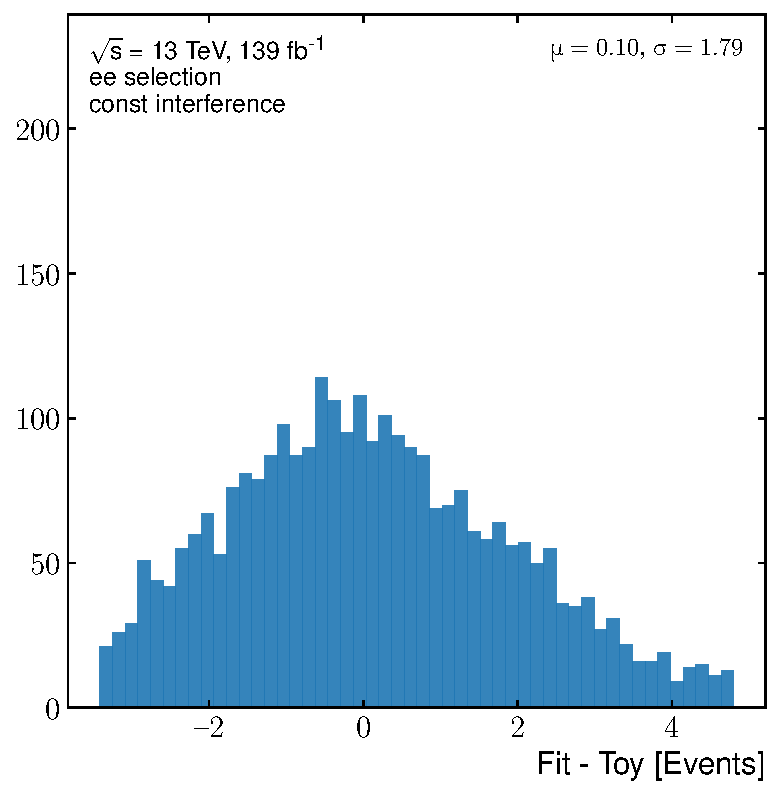
\includegraphics[width=\textwidth]{/Users/Deshan/Documents/PhD/thesis/Thesis/figures/analysis/bkgmodel/uncertainties/fitSs-ee-const.pdf}
        \label{fig:bkgmodel:toyss1}
    \end{subfigure}
    \begin{subfigure}[b]{0.49\textwidth}
        \centering
        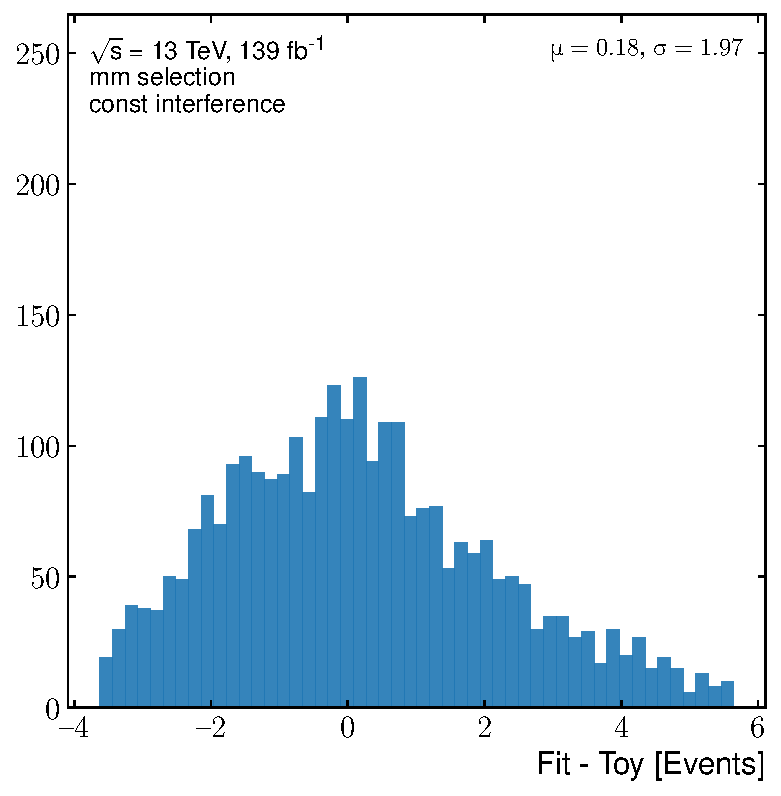
\includegraphics[width=\textwidth]{/Users/Deshan/Documents/PhD/thesis/Thesis/figures/analysis/bkgmodel/uncertainties/fitSs-mm-const.pdf}
        \label{fig:bkgmodel:toyss2}
    \end{subfigure}
    \begin{subfigure}[b]{0.49\textwidth}
        \centering
        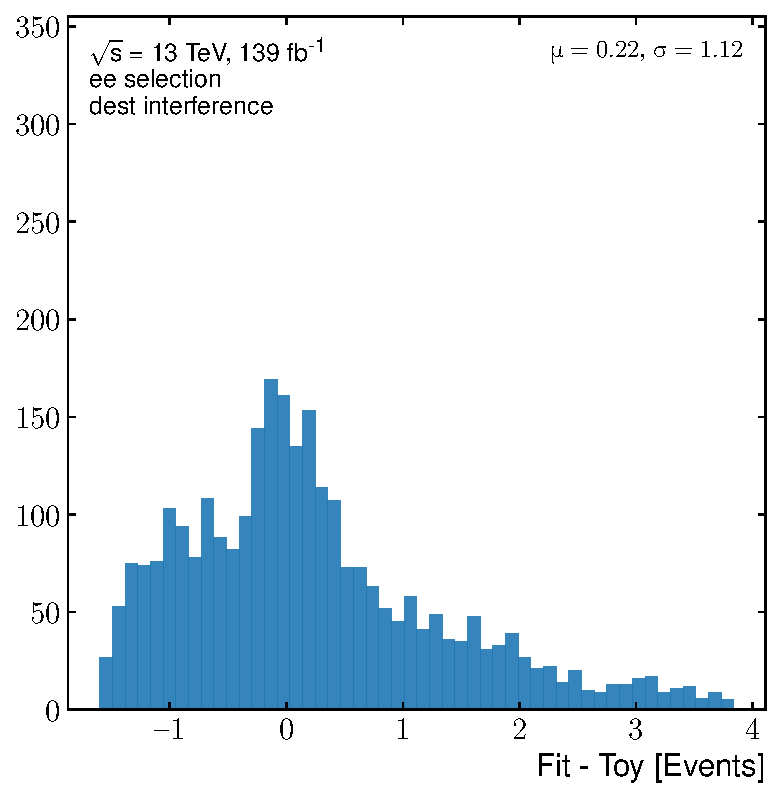
\includegraphics[width=\textwidth]{/Users/Deshan/Documents/PhD/thesis/Thesis/figures/analysis/bkgmodel/uncertainties/fitSs-ee-dest.pdf}
        \label{fig:bkgmodel:toyss3}
    \end{subfigure}
    \begin{subfigure}[b]{0.49\textwidth}
        \centering
        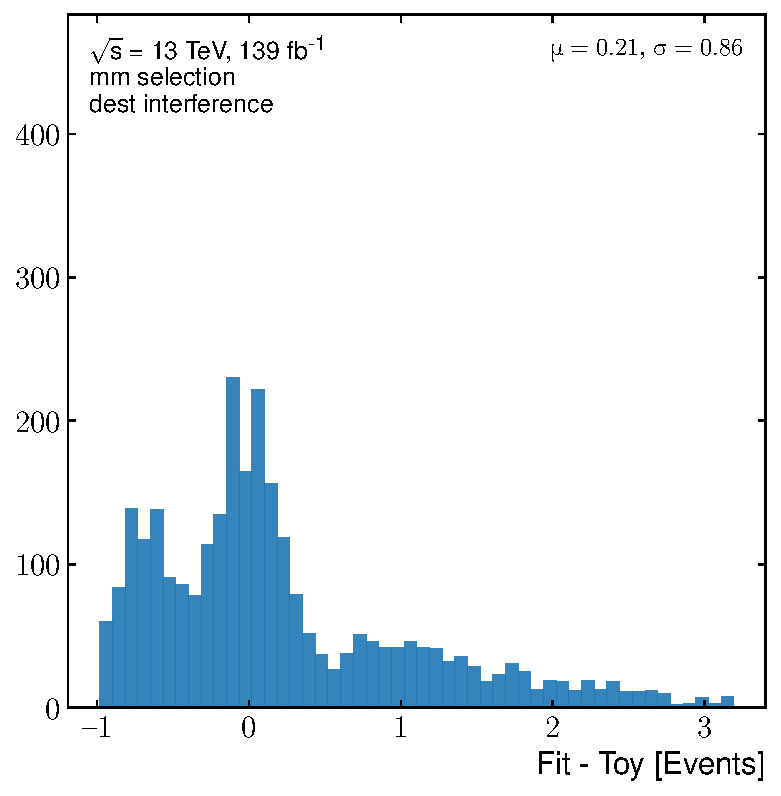
\includegraphics[width=\textwidth]{/Users/Deshan/Documents/PhD/thesis/Thesis/figures/analysis/bkgmodel/uncertainties/fitSs-mm-dest.pdf}
        \label{fig:bkgmodel:toyss4}
    \end{subfigure}
    \caption[Distributions of extrapolation from fit to poisson distributed toys generated in the CR]{Distribution of the difference between the expected background in the SR from fits to poisson generated toys and the background estimation from the toy. The toys have been generated from the fit to the data in the CR. The mean and standard deviation of each distribution is also shown. The constructive (top) and destructive (bottom) SRs for the electron (left) and muon (right) channels are shown.}
    \label{fig:bkgmodel:toyss}
\end{figure}

\subsection{Control region bias uncertainty}\label{sec:uncertBkgmodel:crbu}
The \emph{CR bias uncertainty}, \CRBU, on the expected background quantifies the residual difference between the two functions, with and without the signal component, described in \cref{sec:modelchoice,sec:sigmodel}. Possible signals in data can result in the background estimate from the background-only function being biased. Whereas, the signal+background function is unaffected by the presence of signals. Using simulated samples, the difference between in two models is negligible by construction due to the optimisation of the CR choice. However, when fitting data, small differences between the two functions can be present. The difference is taken as an additional uncertainty on the background estimate. The uncertainty attempts to quantify the degree to which signal-like shapes exist in data for a given CR choice. 

The \CRBU is measured by fitting both the background-only and signal+background functions to data in the CR and extrapolating the background components of the two models to the SR. The background estimate is calculated by integrating the extrapolation in the SR. The difference between the resulting background estimates from the two functions is used as the \CRBU. 

\section{Signal yield uncertainties}\label{sec:uncertBkgmodel:signalyield}
The expected number of simulated CI signal events is used in the statistical analysis to produce results in terms of CI interaction models. The simulated contact interaction expected events in the SR are also affected by the theoretical and experimental uncertainties. The expected signal yield is obtained by integrating the simulated signal in the SR. An uncertainty is assigned to the expected yield by summing in quadrature the uncertainties associated with the signal yield. The theoretical and experimental uncertainties are treated separately and obtained from the procedure described in \cref{chap:sysmc}. Only the experimental uncertainties are used in the statistical analysis. Whereas, the theoretical uncertainties are only shown in the results section as numbers of events. 

\section{Summary of uncertainties}\label{sec:uncertBkgmodel:summary}

The relative uncertainty on both the background estimate and expected signal yield is summarised in \cref{tab:summaryUncerts}. Due to the smaller size of the destructive SRs, there is a smaller expected number of background events, which results in larger relative uncertainties in the SRs. The \CRBU has a minimal impact on the statistical analysis, and the most significant impact is from the \STATU. The signal uncertainties are shows for a \SI{30}{\tera\electronvolt}, this signal was chosen as it is close to the expected sensitivity of the analysis for the constructive and destructive interference models. Additionally, there is only negligible differences between the uncertainties for signal models $\pm \SI{20}{\tera\electronvolt}$.

\begin{table}[htp]
    \begin{center}
    \begingroup
    \setlength{\tabcolsep}{10pt} % Default value: 6pt
    \renewcommand{\arraystretch}{1.5} % Default value: 1
    {\small
    \begin{tabular}{l l | c c c | c c}
    \toprule
            &              & \multicolumn{3}{c|}{Background uncertainties} & \multicolumn{2}{c}{Signal uncertainties}\\
    Channel & Interference & \STATU & \ISSU & \CRBU & \EXPE & \THEO \\
    \hline
    \ee     & Constructive & 20\% & 4\%  & 2\% & 8\%                               & \footnotesize{$^{+11\%}_{-10\%}$}\\
    \ee     & Destructive  & 61\% & 8\% & 1\% & 8\%                               & \footnotesize{$^{+14\%}_{-13\%}$}\\
    $\mumu$ & Constructive & 21\% & 6\%  & 2\% & \footnotesize{$^{+20\%}_{-17\%}$} & \footnotesize{$^{+10\%}_{-9\%}$}\\
    $\mumu$ & Destructive  & 58\% & 24\% & 4\% & \footnotesize{$^{+27\%}_{-22\%}$} & \footnotesize{$^{+13\%}_{-12\%}$}\\
    \bottomrule
    \end{tabular}
    }
    \endgroup
    \end{center}
    \caption[Summary of the relative uncertainties on the background estimate and signal yield in each SR]{Summary of the relative uncertainties on the background estimate and signal in each SR, where \STATU is the ``statistical uncertainty of the fit'', \ISSU is the ``induced spurious signal uncertainty'' and \CRBU is the ``control region bias uncertainty''. Experimental and theoretical uncertainties are shown as well with the latter averaged across CI chirality scenarios and quoted for $\Lambda=30$~TeV only.}
    \label{tab:summaryUncerts}
\end{table}